\documentclass[border=2pt]{standalone}
\usepackage{tikz}
\usetikzlibrary{arrows.meta,positioning,calc,fit,backgrounds,shapes.geometric}
\usepackage{amsmath,amssymb}
\usepackage{times}
\definecolor{ink}{HTML}{243447}
\definecolor{cA}{HTML}{4477AA}
\definecolor{cB}{HTML}{CC6677}
\definecolor{cAu}{HTML}{44AA99}
\definecolor{cS}{HTML}{CCAA33}
\definecolor{grn}{HTML}{228833}
\definecolor{rose}{HTML}{AA3377}
\definecolor{inst}{HTML}{F2E3B3}
\tikzset{
 pap/.style={circle,draw=ink,line width=.6pt,minimum size=15pt,inner sep=0pt,font=\scriptsize\bfseries,text=white},
 aut/.style={rectangle,draw=ink,line width=.6pt,minimum size=13pt,inner sep=0pt,fill=cAu,font=\scriptsize\bfseries,text=white},
 sub/.style={diamond,draw=ink,line width=.6pt,minimum size=17pt,inner sep=0pt,fill=cS,font=\scriptsize\bfseries,text=white},
 gone/.style={draw=ink!35,fill=ink!8,text=ink!40,dashed},
 ed/.style={draw=ink,line width=.7pt},
 msg/.style={-{Stealth[length=4pt]},line width=.9pt,draw=rose},
 ptitle/.style={font=\footnotesize\bfseries,text=ink,anchor=west},
 note/.style={font=\scriptsize,text=ink,align=center},
}

\definecolor{fcF}{HTML}{AA3377}
\definecolor{fcG}{HTML}{EE7733}
\definecolor{lrn}{HTML}{CC3311}
\tikzset{
 stage/.style={draw=ink!45,rounded corners=3pt,line width=.6pt,anchor=north west,fill=white},
 stnum/.style={circle,fill=ink,text=white,font=\footnotesize\bfseries,inner sep=1.3pt},
 sname/.style={font=\small\bfseries,text=ink,anchor=west},
 lab/.style={font=\footnotesize,text=ink},
 learn/.style={draw=lrn,dashed,line width=.8pt,rounded corners=2pt,fill=lrn!5,font=\footnotesize,text=ink,inner sep=2.5pt,align=center},
 est/.style={rectangle,draw=grn,fill=grn!15,line width=.6pt,minimum size=7pt,inner sep=0pt},
 vec/.style={draw=ink,fill=#1,minimum width=4pt,minimum height=9pt,inner sep=0pt},
 flow/.style={-{Stealth[length=5pt]},line width=1.2pt,draw=ink!55},
 arr/.style={-{Stealth[length=3.5pt]},line width=.7pt,draw=ink!70},
 mp/.style={-{Stealth[length=3.5pt]},grn,line width=.9pt},
 ribbon/.style={line width=9pt,line cap=round,line join=round,draw=#1,draw opacity=.28},
 walk/.style={-{Stealth[length=4pt]},line width=1pt,draw=#1},
 nedge/.style={draw=ink!55,line width=.6pt},
 cpl/.style={line width=.65pt,draw=#1},
 pS/.style={pap,minimum size=14pt},
 aS/.style={aut,minimum size=12pt},
 sS/.style={sub,minimum size=15pt},
}
\newcommand{\bars}[4]{\foreach \k in {1,...,#3}{\node[vec=#4] at ($(#1)+(#2)+(\k*0.15,0)$) {};}}
\begin{document}
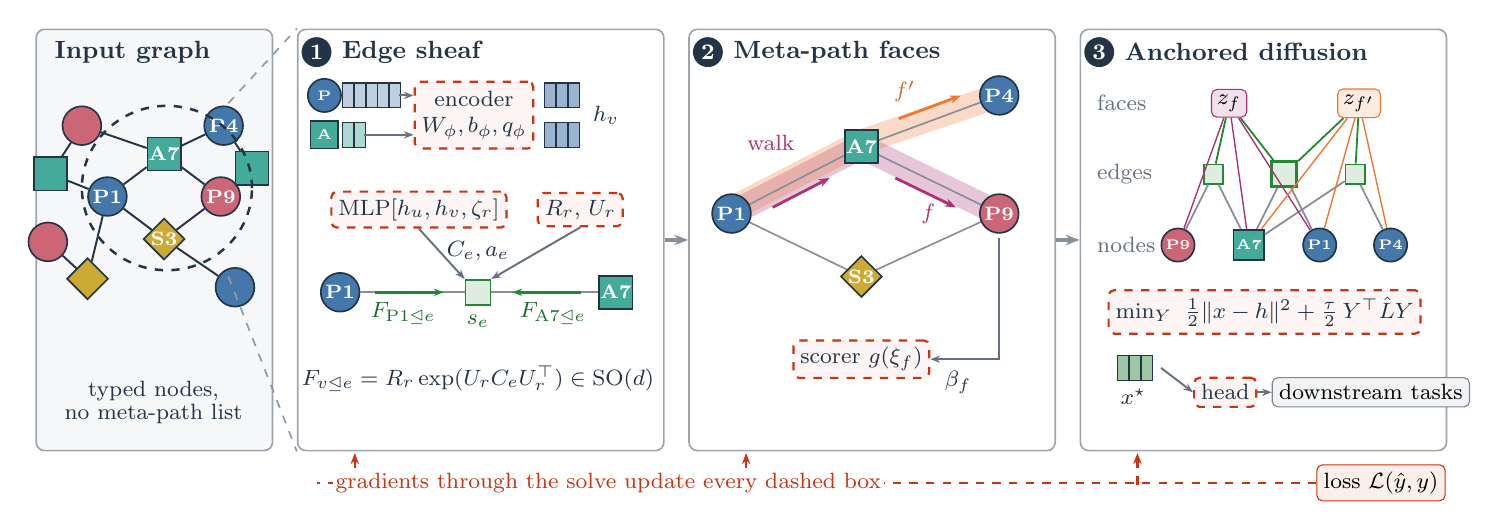
\begin{tikzpicture}
\def\WI{3.0}\def\WP{4.65}\def\G{0.32}\def\H{5.35}
\pgfmathsetmacro{\xA}{\WI+\G}\pgfmathsetmacro{\xB}{\xA+\WP+\G}\pgfmathsetmacro{\xC}{\xB+\WP+\G}
\node[stage,minimum width=\WI cm,minimum height=\H cm,fill=ink!4] (BI) at (0,0) {};
\node[sname] at (0.12,-0.3) {Input graph};
\foreach \i/\x/\t in {1/\xA/Edge sheaf,2/\xB/Meta-path faces,3/\xC/Anchored diffusion}{
  \node[stage,minimum width=\WP cm,minimum height=\H cm] (B\i) at (\x,0) {};
  \node[stnum] at ($(B\i.north west)+(0.25,-0.3)$) {\i};
  \node[sname] at ($(B\i.north west)+(0.45,-0.3)$) {\t};
}
% ================= input
\begin{scope}[shift={(0.05,-0.55)},scale=0.72]
 \node[pS,fill=cA] (iP1) at (1.2,-2.2) {P1};
 \node[aS] (iA7) at (2.2,-1.45) {A7};
 \node[sS] (iS3) at (2.2,-2.95) {S3};
 \node[pS,fill=cB] (iP9) at (3.2,-2.2) {P9};
 \node[pS,fill=cA] (iP4) at (3.25,-0.95) {P4};
 \node[pS,fill=cB] (iP2) at (0.75,-0.95) {};
 \node[aS] (iA2) at (0.2,-1.8) {};
 \node[pS,fill=cA] (iP6) at (3.45,-3.8) {};
 \node[sS] (iS4) at (0.85,-3.65) {};
 \node[pS,fill=cB] (iP7) at (0.15,-3.0) {};
 \node[aS] (iA5) at (3.75,-1.7) {};
 \draw[ed] (iP1)--(iA7) (iA7)--(iP9) (iA7)--(iP4) (iP1)--(iS3) (iS3)--(iP9)
   (iA2)--(iP2) (iA2)--(iP1) (iS3)--(iP6) (iP2)--(iA7) (iS4)--(iP7) (iS4)--(iP1) (iA5)--(iP9) (iA5)--(iP4);
 \draw[ink,dashed,line width=.9pt] (2.25,-2.05) ellipse (1.5 and 1.45);
\end{scope}
\node[lab,align=center] at (\WI/2,-4.75) {typed nodes,\\[-1pt]no meta-path list};
\draw[dashed,ink!50,line width=.6pt] (2.45,-0.95)--(B1.north west);
\draw[dashed,ink!50,line width=.6pt] (2.45,-3.15)--(B1.south west);
% ================= 1 edge sheaf
\begin{scope}[shift={(\xA,0)}]
 % type encoder
 \node[pS,fill=cA,minimum size=12pt,font=\tiny\bfseries] (eP) at (0.35,-0.85) {P};
 \node[aS,minimum size=10pt,font=\tiny\bfseries] (eA) at (0.35,-1.35) {A};
 \bars{eP}{0.15,0}{5}{cA!35} \bars{eA}{0.15,0}{2}{cAu!45}
 \node[learn,minimum width=1.25cm,minimum height=0.85cm] (enc) at (2.25,-1.1) {encoder\\$W_{\phi},b_{\phi},q_{\phi}$};
 \draw[arr] (1.3,-0.85)--(enc.west|-0,-0.85); \draw[arr] (0.85,-1.35)--(enc.west|-0,-1.35);
 \bars{enc.east}{0.05,0.25}{3}{cA!55} \bars{enc.east}{0.05,-0.25}{3}{cA!55}
 \node[lab,anchor=west] at ($(enc.east)+(0.62,0)$) {$h_v$};
 % edge with maps
 \node[pS,fill=cA] (aP1) at (0.55,-3.35) {P1};
 \node[aS] (aA7) at (4.05,-3.35) {A7};
 \node[est,minimum size=9pt] (se) at (2.3,-3.35) {};
 \draw[nedge] (aP1)--(se)--(aA7);
 \draw[mp] ($(aP1)!0.25!(se)$)--($(aP1)!0.75!(se)$); \draw[mp] ($(aA7)!0.25!(se)$)--($(aA7)!0.75!(se)$);
 \node[lab,text=grn!80!black,anchor=north] at (se.south) {$s_e$};
 \node[lab,text=grn!80!black] at (1.35,-3.62) {$F_{\mathrm{P1}\trianglelefteq e}$};
 \node[lab,text=grn!80!black] at (3.25,-3.62) {$F_{\mathrm{A7}\trianglelefteq e}$};
 \node[learn] (mlp) at (1.55,-2.3) {MLP$[h_u,h_v,\zeta_r]$};
 \node[learn] (frm) at (3.6,-2.3) {$R_r,\,U_r$};
 \draw[arr] (mlp.south)--node[lab,right=-1pt,pos=.45]{$C_e,a_e$}(se.north west);
 \draw[arr] (frm.south)--(se.north east);
 \node[lab] at (2.3,-4.45) {$F_{v\trianglelefteq e}=R_r\exp(U_rC_eU_r^{\top})\in\mathrm{SO}(d)$};
\end{scope}
% ================= 2 meta-path faces
\begin{scope}[shift={(\xB,0)}]
 \coordinate (P1) at (0.55,-2.35); \coordinate (A7) at (2.2,-1.5); \coordinate (P9) at (3.95,-2.35);
 \coordinate (P4) at (3.95,-0.85); \coordinate (S3) at (2.2,-3.15);
 \draw[ribbon=fcF] (P1)--(A7)--(P9);
 \draw[ribbon=fcG] ($(P1)+(0,0.06)$)--($(A7)+(0,0.06)$)--(P4);
 \draw[nedge] (P1)--(A7) (A7)--(P9) (A7)--(P4) (P1)--(S3) (S3)--(P9);
 \node[pS,fill=cA] (bP1) at (P1) {P1}; \node[aS] (bA7) at (A7) {A7}; \node[pS,fill=cB] (bP9) at (P9) {P9};
 \node[pS,fill=cA] (bP4) at (P4) {P4}; \node[sS] (bS3) at (S3) {S3};
 \draw[walk=fcF] ($(P1)!0.28!(A7)+(0.06,-0.16)$)--($(P1)!0.72!(A7)+(0.06,-0.16)$);
 \draw[walk=fcF] ($(A7)!0.28!(P9)+(-0.06,-0.16)$)--($(A7)!0.72!(P9)+(-0.06,-0.16)$);
 \draw[walk=fcG] ($(A7)!0.3!(P4)+(-0.05,0.16)$)--($(A7)!0.75!(P4)+(-0.05,0.16)$);
 \node[lab,text=fcF,font=\footnotesize\bfseries] at (3.05,-2.35) {$f$};
 \node[lab,text=fcG!90!black,font=\footnotesize\bfseries] at (2.75,-0.8) {$f'$};
 \node[learn] (gsc) at (2.2,-4.2) {scorer $g(\xi_f)$};
 \draw[arr] ($(bP9.south)+(0,-0.05)$) |- (gsc.east);
 \node[lab,anchor=west] at ($(gsc.east)+(0.06,-0.3)$) {$\beta_f$};
 \node[lab,text=fcF] at (1.05,-1.45) {walk};
\end{scope}
% ================= 3 anchored diffusion
\begin{scope}[shift={(\xC,0)}]
 \node[lab,anchor=west,text=ink!70] at (0.1,-0.95) {faces};
 \node[lab,anchor=west,text=ink!70] at (0.1,-1.85) {edges};
 \node[lab,anchor=west,text=ink!70] at (0.1,-2.75) {nodes};
 \node[draw=fcF,fill=fcF!15,rounded corners=2pt,font=\footnotesize,inner sep=2pt] (zf) at (1.9,-0.95) {$z_f$};
 \node[draw=fcG,fill=fcG!15,rounded corners=2pt,font=\footnotesize,inner sep=2pt] (zg) at (3.55,-0.95) {$z_{f'}$};
 \node[pS,fill=cB,minimum size=12pt,font=\tiny\bfseries] (n9) at (1.25,-2.75) {P9};
 \node[aS,minimum size=11pt,font=\tiny\bfseries] (n7) at (2.15,-2.75) {A7};
 \node[pS,fill=cA,minimum size=12pt,font=\tiny\bfseries] (n1) at (3.05,-2.75) {P1};
 \node[pS,fill=cA,minimum size=12pt,font=\tiny\bfseries] (n4) at (3.95,-2.75) {P4};
 \node[est] (e97) at (1.7,-1.85) {}; \node[est,minimum size=9pt,line width=1pt] (e71) at (2.6,-1.85) {}; \node[est] (e74) at (3.5,-1.85) {};
 \draw[cpl=ink!55] (n9)--(e97) (n7)--(e97) (n7)--(e71) (n1)--(e71) (n7)--(e74) (n4)--(e74);
 \draw[cpl=grn] (zf)--(e97) (zf)--(e71) (zg)--(e71) (zg)--(e74);
 \foreach \n in {n9,n7,n1} \draw[cpl=fcF,line width=.5pt] (zf)--(\n);
 \foreach \n in {n1,n7,n4} \draw[cpl=fcG,line width=.5pt] (zg)--(\n);
 \node[learn,font=\footnotesize] (sol) at (2.35,-3.6) {$\min_Y\ \tfrac12\|x-h\|^2+\tfrac{\tau}{2}\,Y^{\top}\hat LY$};
 \bars{sol.south west}{0.05,-0.42}{3}{grn!45}
 \node[lab] at ($(sol.south west)+(0.33,-0.78)$) {$x^\star$};
 \node[learn] (head) at (1.85,-4.62) {head};
 \draw[arr] ($(sol.south west)+(0.68,-0.42)$)--(head.west);
 \node[draw=ink!60,rounded corners=2pt,fill=ink!6,font=\footnotesize,inner sep=2.5pt] (ds) at (3.7,-4.62) {downstream\\[-2pt] tasks};
 \draw[arr] (head.east)--(ds.west);
\end{scope}
\draw[flow] (B1.east)--(B2.west); \draw[flow] (B2.east)--(B3.west);
% ================= loss
\pgfmathsetmacro{\yL}{-\H-0.42}
\node[draw=lrn,fill=lrn!8,rounded corners=2pt,font=\footnotesize,inner sep=2.5pt,anchor=east] (loss) at (\xC+\WP,\yL) {loss $\mathcal{L}(\hat y,y)$};
\draw[lrn,dashed,line width=.8pt] (loss.west)--(\xA+0.25,\yL);
\foreach \b in {B1,B2,B3}{\draw[-{Stealth[length=4pt]},lrn,dashed,line width=.8pt] ($(\b.south)+(-1.6,-0.42)$)--($(\b.south)+(-1.6,-0.02)$);}
\node[font=\footnotesize,text=lrn,anchor=west,fill=white,inner sep=1pt] at (\xA+0.45,\yL) {gradients through the solve update every dashed box};
\end{tikzpicture}
\end{document}
